% Tento soubor nahraďte vlastním souborem s přílohami (nadpisy níže jsou pouze pro příklad)
% This file should be replaced with your file with an appendices (headings below are examples only)

% Umístění obsahu paměťového média do příloh je vhodné konzultovat s vedoucím
% Placing of table of contents of the memory media here should be consulted with a supervisor
%\chapter{Obsah přiloženého paměťového média}

%\chapter{Manuál}

%\chapter{Konfigurační soubor} % Configuration file

%\chapter{RelaxNG Schéma konfiguračního souboru} % Scheme of RelaxNG configuration file

%\chapter{Plakát} % poster


\chapter{Obsah DVD} % poster

\begin{description}
	\item[/.*] - soubory s informacemi k nastavení programu a spouštěcí soubor.
	\item[/build/] - zkomprimované zdrojové soubory pro rychlejší načítání na webu.	
	\item[/data/] - multimediální soubory.	
	\item[/doc/] - soubory s technickou zprávou, obrázky a zdrojovými soubory.	
	\item[/src/] - složka se zdrojovými kódy programu strukturovaná na:	
		\begin{description}
			\item[/js/] - javascriptové knihovny a hlavní zdrojový soubor programu.
			\item[/img/] - obrázky programu.
			\item[/css/] - kaskádové styly programu.
		\end{description}
\end{description}

%\dirtree{%
%	.1 /.
%	.2 doc \ldots{}  This directory holds executable files {.}.
%	.2 src \ldots{}  This directory holds executable files {.}.
%		.3 js \ldots{}  This directory holds executable files {.}. 
%		.3 img \ldots{}  This directory holds executable files {.}. 
%		.3 css \ldots{}  This directory holds executable files {.}. 
%	.2 data \ldots{}  This directory holds executable files {.}. 
%	.2 bin.
%}
 
\chapter{Obrázky z programu} % poster
\begin{figure}[h]
	\label{img:12}
	\centering
	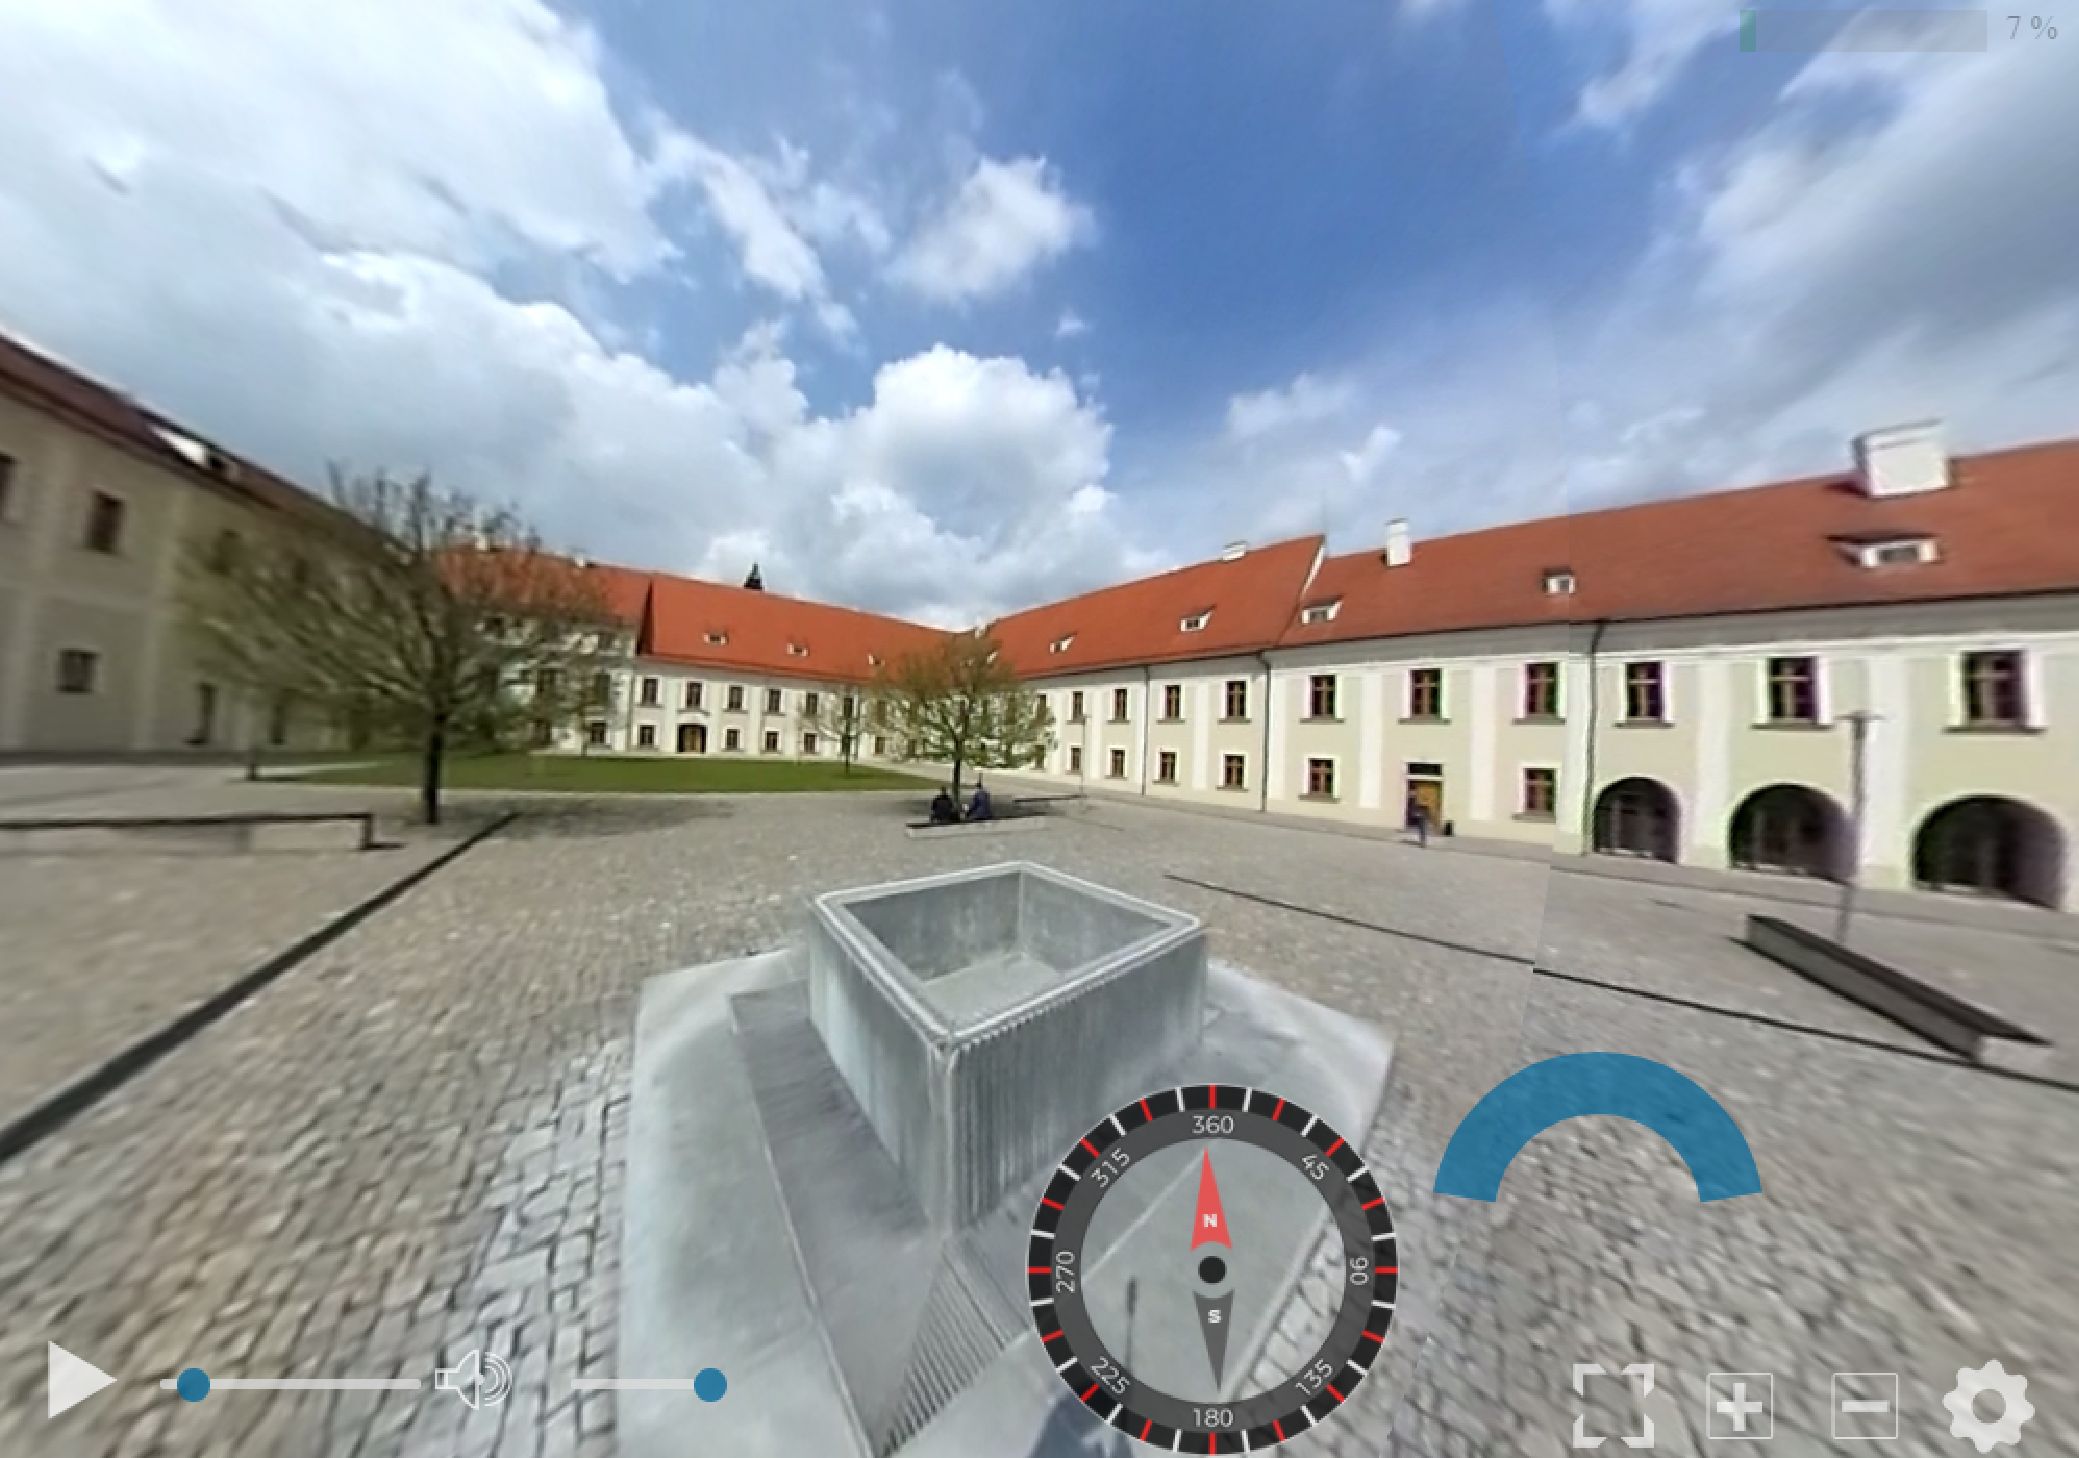
\includegraphics[scale=1.0,angle=0,width=1.0\linewidth]{obrazky-figures/priloha_b1}
	\caption{Ukázka prohlížení v režimu rybího oka.}
\end{figure}

\newpage


\begin{figure}[h]
	\label{img:13}
	\centering
	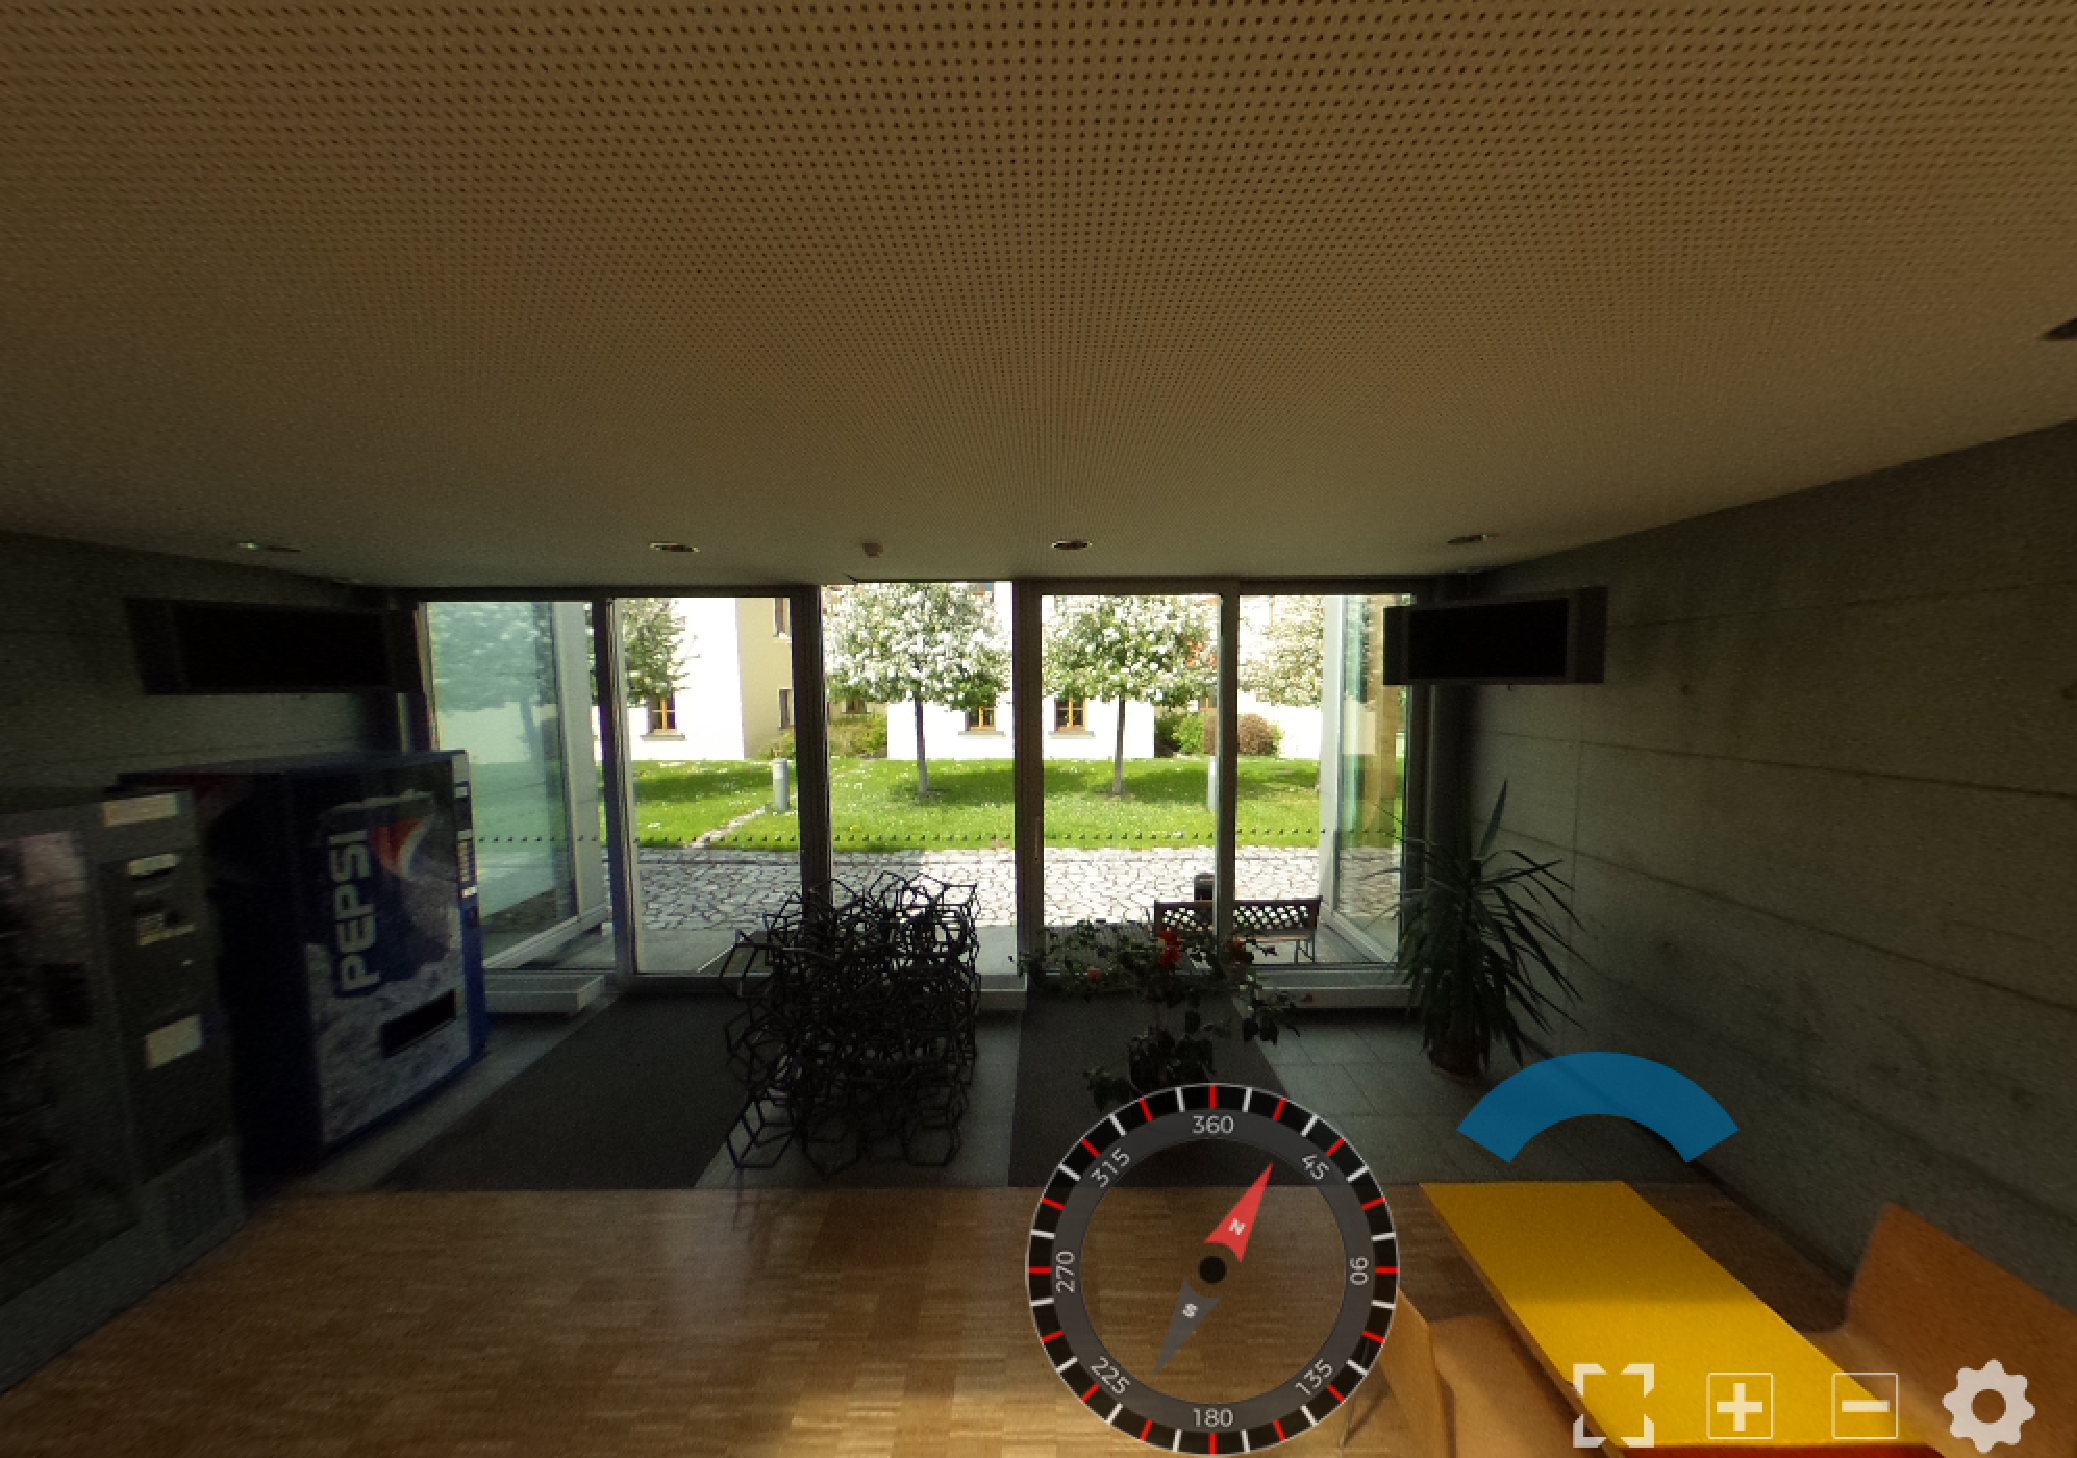
\includegraphics[scale=1.0,angle=0,width=1.0\linewidth]{obrazky-figures/priloha_b2}
	\caption{Sférická fotka v ekvidistantním režimu.}
\end{figure}

